\newcommand{\hsbind}{\mathbin{\gg\!=}}
\newcommand{\apl}{\mathbin{\ll\!\!\cdot}}
\newcommand{\apr}{\mathbin{\cdot\!\!\gg}}
\newcommand{\aplr}{\mathbin{\ll\!\!\cdot\!\!\gg}}
\newcommand{\cons}{\mathbin{::}}
\newcommand{\cat}{\mathbin{+\mkern-10mu+}}

\newcommand{\abs}[1]{\textsc{#1}}
\newcommand{\obj}[1]{\textbf{#1}}
\newcommand{\sem}[1]{\llbracket #1 \rrbracket}
\newcommand{\lex}[2]{\sem{\abs{#1}} &:= #2}

\newcommand{\dand}{\mathbin{\overline{\land}}}
\newcommand{\dnot}{\mathop{\overline{\lnot}}}
\newcommand{\dor}{\mathop{\overline{\lor}}}
\newcommand{\dimpl}{\mathbin{\overline{\to}}}
\newcommand{\dexists}{\mathop{\overline{\exists}}}
\newcommand{\dforall}{\mathop{\overline{\forall}}}

\newcommand{\limp}{\mathbin{{-}\mkern-3.5mu{\circ}}}

\newcommand{\llbparenthesis}{\vcenter{\hbox{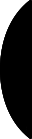
\includegraphics{symbols/llbparenthesis.png}}}}
\newcommand{\rrbparenthesis}{\vcenter{\hbox{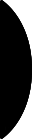
\includegraphics{symbols/rrbparenthesis.png}}}}
\newcommand{\lban}{\llparenthesis \,}
\newcommand{\rban}{\, \rrparenthesis}
\newcommand{\lbban}{\llbparenthesis \,}
\newcommand{\rbban}{\, \rrbparenthesis}
\newcommand{\banana}[1]{\lban #1 \rban}
\newcommand{\bbanana}[1]{\lbban #1 \rbban}
\newcommand{\cherry}{\rotatebox[origin=c]{270}{$\limp$}}

\newcommand{\lam}[2]{\lambda #1.\, #2}
\newcommand{\ap}[2]{#1\,#2}
\newcommand{\op}[1]{\mathtt{#1}}
\newcommand{\onto}[1]{#1 \mathalpha{:\,}}
\newcommand{\typedop}[3]{\op{#1} : #2 \rightarrowtail #3}
\newcommand{\typedopg}[3]{#1 : #2 \rightarrowtail #3}
\newcommand{\row}[2]{\{ #1 \mathrel{|} #2 \}}

\newcommand{\CC}{\mathcal{C}}
\newcommand{\FF}{\mathcal{F}}
\newcommand{\XX}{\mathcal{X}}
\newcommand{\EE}{\mathcal{E}}
\newcommand{\TT}{\mathcal{T}}
\newcommand{\PP}{\mathcal{P}}

\newcommand{\FV}{\operatorname{FV}}

\newcommand{\subst}[3]{#1[#2 \coloneqq #3]}

\newcommand{\syntclos}[1]{\mathbin{[#1]}}

\newtheorem*{definition}{Definition}
\newtheorem*{observation}{Observation}

\newcommand{\cibanana}{\banana{(\onto{\op{op}_i} M_i)_{i \in I},\ \onto{\eta} M_\eta}}
\newcommand{\cdbanana}{\banana{\onto{\op{op}_1} M_1,\ \dots,\ \onto{\op{op}_n} M_n,\ \onto{\eta} M_\eta}}

\newcommand{\cibbanana}{\bbanana{(\onto{\op{op}_i} M_i)_{i \in I},\ \onto{\eta} M_\eta}}

\newcommand{\TODO}[1]{\textcolor{red}{\textbf{TODO}: #1}}

\newcommand{\relR}{\mathbin{R}}

\newcommand{\swap}{\mathbin{\textbf{swap}}}

\newcommand{\tto}{\twoheadrightarrow}

\mathchardef\mhyphen="2D
